\documentclass[10pt]{beamer}
\usetheme{default}

\title{Anforderungen für OpenSlides 4}
\author{}
\date{}

\beamertemplatenavigationsymbolsempty
\setbeamertemplate{footline}[frame number]


\begin{document}
\begin{frame}[plain]
    \maketitle
\end{frame}

\begin{frame}{Übersicht}
	\tableofcontents
\end{frame}

\section{Gremienmanagement}
\begin{frame}{Gremienmanagement}
	\begin{itemize}
		\item Metaebene: \textbf{Organisation} enthält \textbf{Gremien}
		\item Gremien enthalten \textbf{Veranstaltungen} ($\hat{=}$ OS3-Instanzen)
		\item Zentrale \textbf{Nutzerverwaltung}
	\end{itemize}
	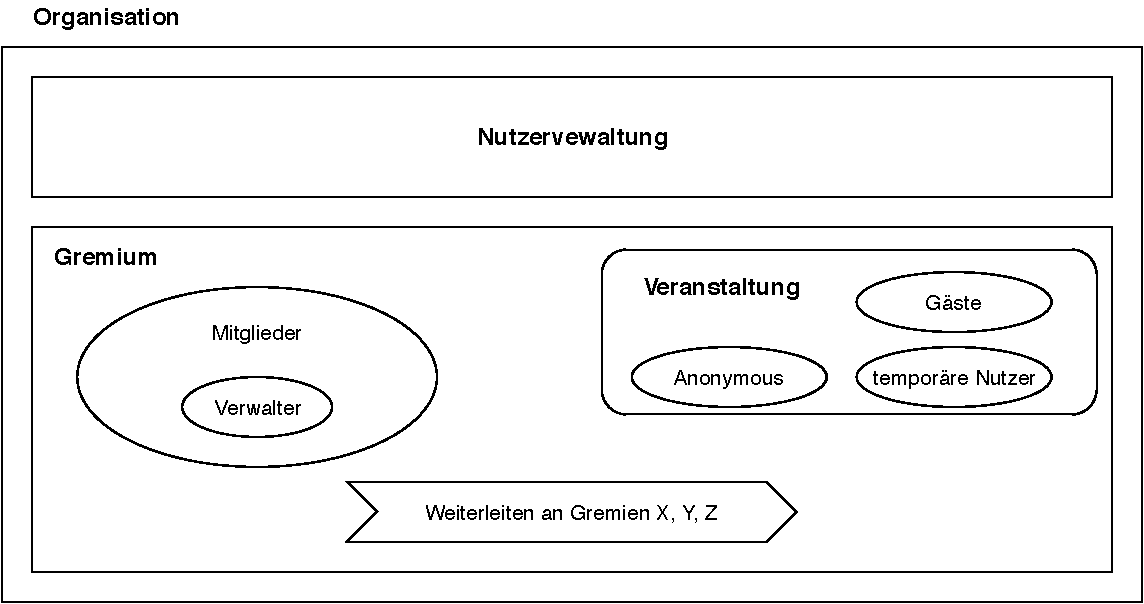
\includegraphics[scale=0.55]{organisation}
\end{frame}

\section{Nutzeranforderungen}
\begin{frame}{Nutzeranforderungen}
	\begin{itemize}
		\item<+-> 2 Millionen Nutzer. Erwartung: Steigende Nutzungszahlen
		\item<+-> Persönliche Benachrichtigungen, mehrere Wege
		\item<+-> Erweiterte persönliche Notizen
		\item<+-> Nutzerspezifische Labels
		\item<+-> Sicherheitszentrale
	\end{itemize}
\end{frame}

\section{Technische Neuerungen}
\begin{frame}{Technische Neuerungen}
	\begin{itemize}
		\item<+-> Import und Export von Veranstaltungen
		\item<+-> History als Backup und Papierkorb
		\item<+-> Logging, Metriken
		\item<+-> Reduzierung von chatty-APIs (u.a. Autoupdates)
		\item<+-> Skalierbarkeit: Unterschiedliche Anforderungen an Systemteile
		\item<+-> TDD und einheitliche Codestandards
	\end{itemize}
\end{frame}

\end{document}
